\section{Experiments}
\label{sec:experiments}

\subsection{Setup}
\label{sec:exp-setup}

Four systems are compared on the protocol of \S\ref{sec:method-protocol}.
\textbf{Part~1} is the template-difference baseline (\S\ref{sec:method-part1}).
\textbf{Part~2} is the official AnomalyDINO reproduction (DINOv2 ViT-S/14 @448, agnostic
preprocessing, PCA foreground mask), verified cell-by-cell against the published pipeline.
\textbf{E1 control} is DINOv2 @448 with the mask disabled -- the identical-scoring
counterpart of our CLIP arm. \textbf{E1 CLIP} is CLIP ViT-B/16 @448, block 9,
\texttt{short\_edge} framing, no mask, with patch tokens extracted and probe-verified as
described in \S\ref{sec:method-e1}. The controlled pair (control vs CLIP) differs \emph{only}
in the encoder; Part~2 differs additionally in preprocessing -- its mask is worth
${\approx}1.3$ image points, measured as official minus control -- and is the complete-system
reference, not a controlled arm.

\subsection{Main results}
\label{sec:exp-main}

\begin{table}[t]
\centering
\caption{Image-level AUROC (\%), mean\,$\pm$\,std over three seeds of the six-category
means. The controlled pair is DINOv2-control vs CLIP; Part~2 adds the official PCA mask and
is a complete-system reference. Best per column in bold.}
\label{tab:image}
\footnotesize
\setlength{\tabcolsep}{2.2pt}
\begin{tabular}{lcccc}
\toprule
Method & 1-shot & 2-shot & 4-shot & 8-shot \\
\midrule
Template diff.\ (Part 1) & 52.00\,\std{1.13} & 54.08\,\std{3.38} & 55.36\,\std{3.22} & 57.96\,\std{0.47} \\
AnomalyDINO (Part 2, masked) & \best{94.61}\,\std{0.84} & \best{95.33}\,\std{0.46} & \best{96.15}\,\std{0.40} & \best{96.62}\,\std{0.57} \\
DINOv2 @448 nomask (ctrl) & 93.34\,\std{0.72} & 94.16\,\std{0.27} & 94.92\,\std{0.49} & 95.37\,\std{0.72} \\
CLIP @448 L9 nomask (E1) & 87.70\,\std{1.24} & 89.22\,\std{0.29} & 89.27\,\std{0.38} & 89.48\,\std{0.23} \\
\bottomrule
\end{tabular}
\end{table}

\begin{table}[t]
\centering
\caption{Pixel-level AUROC (\%), same aggregation as Table~\ref{tab:image}.}
\label{tab:pixel}
\footnotesize
\setlength{\tabcolsep}{2.2pt}
\begin{tabular}{lcccc}
\toprule
Method & 1-shot & 2-shot & 4-shot & 8-shot \\
\midrule
Template diff.\ (Part 1) & 65.06\,\std{0.41} & 64.85\,\std{0.39} & 65.47\,\std{0.29} & 66.14\,\std{0.22} \\
AnomalyDINO (Part 2, masked) & \best{98.08}\,\std{0.05} & \best{98.22}\,\std{0.07} & \best{98.36}\,\std{0.03} & \best{98.47}\,\std{0.01} \\
DINOv2 @448 nomask (ctrl) & 97.06\,\std{0.32} & 97.57\,\std{0.11} & 97.91\,\std{0.06} & 98.16\,\std{0.04} \\
CLIP @448 L9 nomask (E1) & 94.44\,\std{0.10} & 94.97\,\std{0.09} & 95.22\,\std{0.06} & 95.46\,\std{0.05} \\
\bottomrule
\end{tabular}
\end{table}

Under the controlled protocol, replacing DINOv2 with CLIP costs \textbf{5.6 image points at
1-shot} (87.70 vs 93.34) and 2.6 pixel points, and the deficit \textbf{does not close with
more references}: CLIP gains $+1.8$ image points from 1-shot to 8-shot, the DINOv2 control
gains $+2.0$, and the ordering never flips (Tables~\ref{tab:image},~\ref{tab:pixel};
Fig.~\ref{fig:shots}). The few-shot deficit is therefore a property of the features, not of
sample size. The official masked baseline sits another ${\approx}1.3$ image points above the
unmasked control at every shot count, which prices the PCA foreground mask and explains why
it was removed from both controlled arms rather than granted to one.

\begin{figure}[t]
  \centering
  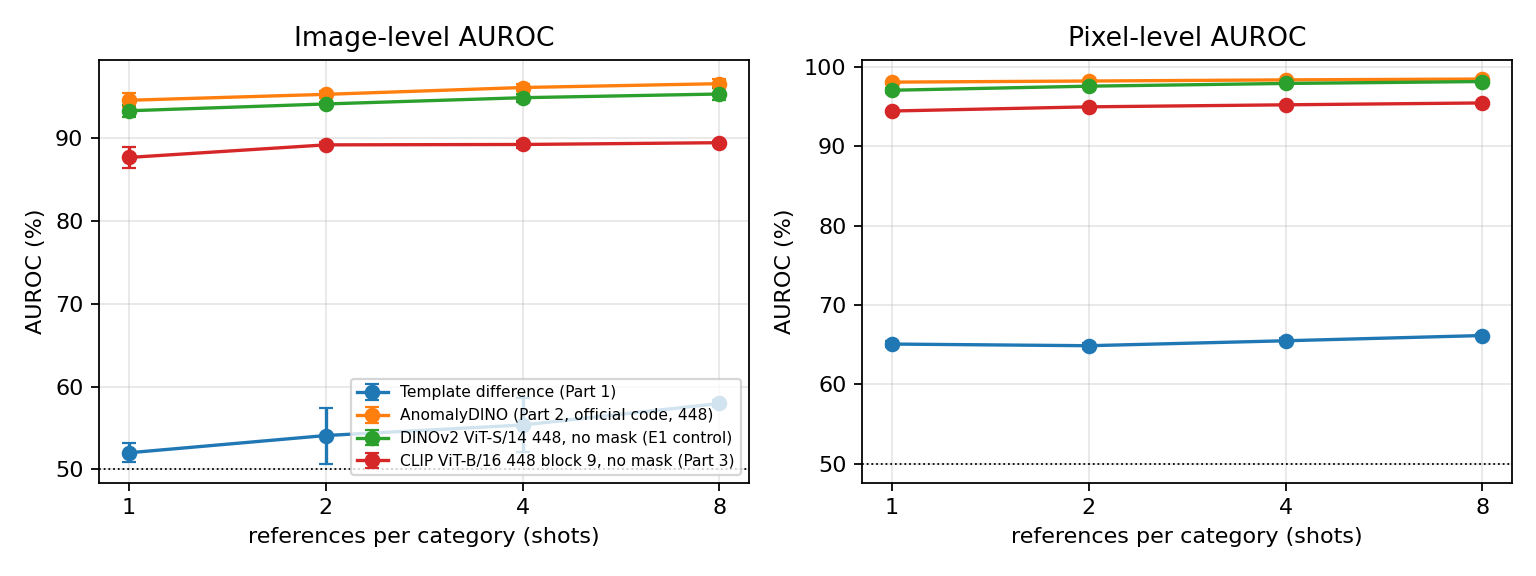
\includegraphics[width=\columnwidth]{figures/auroc_vs_shots.png}
  \caption{Image and pixel AUROC vs number of references, all four systems. The CLIP--DINOv2
  gap is essentially constant in $K$.}
  \label{fig:shots}
\end{figure}

\begin{figure}[t]
  \centering
  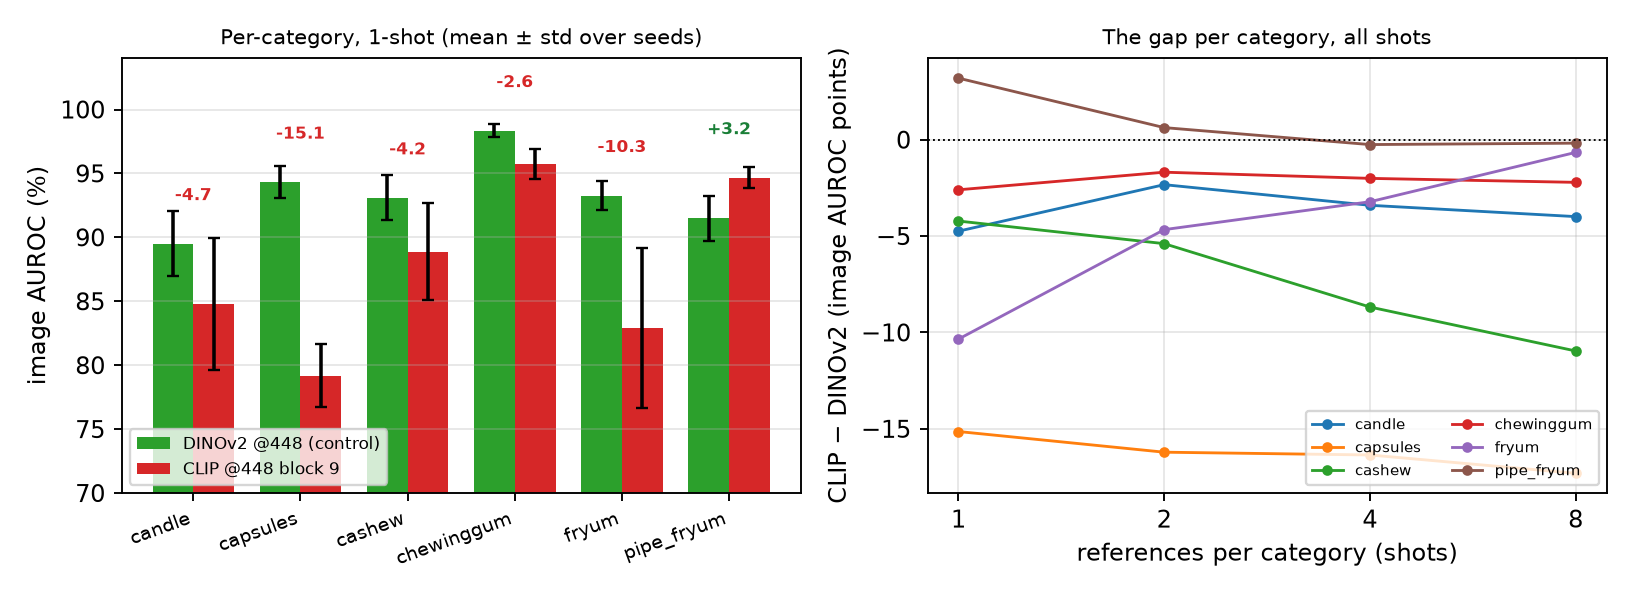
\includegraphics[width=\columnwidth]{figures/per_category_1shot.png}
  \caption{Per-category analysis. Left: 1-shot image AUROC per category (bars, seed std) with
  the CLIP$-$DINOv2 gap annotated. Right: the gap across shot counts. capsules diverges
  ($-15.1 \rightarrow -17.3$), fryum converges ($-10.3 \rightarrow -0.7$), pipe\_fryum is
  reversed ($+3.2$ at 1-shot).}
  \label{fig:percat}
\end{figure}

\subsection{Per-category analysis}
\label{sec:exp-percat}

\begin{table}[t]
\centering
\caption{Per-category gap $\Delta =$ CLIP $-$ DINOv2, image AUROC points (mean over seeds).}
\label{tab:gap}
\small
\begin{tabular}{lrrrr}
\toprule
category & 1-shot & 2-shot & 4-shot & 8-shot \\
\midrule
candle & $-4.7$ & $-2.3$ & $-3.4$ & $-4.0$ \\
capsules & $-15.1$ & $-16.2$ & $-16.4$ & $-17.3$ \\
cashew & $-4.2$ & $-5.4$ & $-8.7$ & $-11.0$ \\
chewinggum & $-2.6$ & $-1.7$ & $-2.0$ & $-2.2$ \\
fryum & $-10.3$ & $-4.7$ & $-3.2$ & $-0.7$ \\
pipe\_fryum & \best{$+3.2$} & $+0.6$ & $-0.3$ & $-0.2$ \\
\bottomrule
\end{tabular}
\end{table}

Three regimes are visible (Table~\ref{tab:gap}, Fig.~\ref{fig:percat}).
\emph{Persistent, large deficits} -- capsules starts 15.1 behind and \emph{widens} to 17.3;
its defects are sub-patch-scale colour/end-cap anomalies where CLIP's 16-px,
language-aligned tokens keep firing on normal background variation (\S\ref{sec:exp-mech}).
\emph{Diverging trends} -- fryum starts 10.3 behind but converges to $-0.7$ at 8-shot, the
only category where more references nearly close the gap. \emph{A reversal} -- pipe\_fryum is
the one category where CLIP is ahead at 1-shot ($+3.2$) and statistically tied at 4/8-shot:
on highly regular, near-periodic objects the globally aligned features are not strictly
worse. An aggregate-only table would hide all three; the reversal and the fryum pixel tie
(CLIP matches the control's pixel AUROC there while trailing 10.3 on image AUROC) are the
quantitative footing for the complementarity claim that the fusion experiments test.

\subsection{Why CLIP trails: anisotropy and map variance}
\label{sec:exp-mech}

The mechanism was measured, not assumed. Patch features inside one image are far more
anisotropic in CLIP's last block -- mean pairwise cosine similarity 0.57--0.67 against 0.36
for DINOv2 L12 -- so nearest-neighbour \emph{distances} compress unevenly across the image.
The layer sweep found block 9 the least anisotropic of \{6, 9, 12\} and the best under the
frozen framing. The direct visual consequence is in Fig.~\ref{fig:heatmaps}: DINOv2's
distance field is near-flat over the background with isolated hotspots, while CLIP's block-9
map is high-variance everywhere, so large areas of \emph{normal} background sit close to the
decision threshold (candle: CLIP's calibration threshold 0.355 vs DINOv2's 0.269 at the same
nominal operating point). Small defects then drown in background variance -- exactly the
capsules ($-15.1$) and fryum ($-10.3$) regime.

\begin{figure}[t]
  \centering
  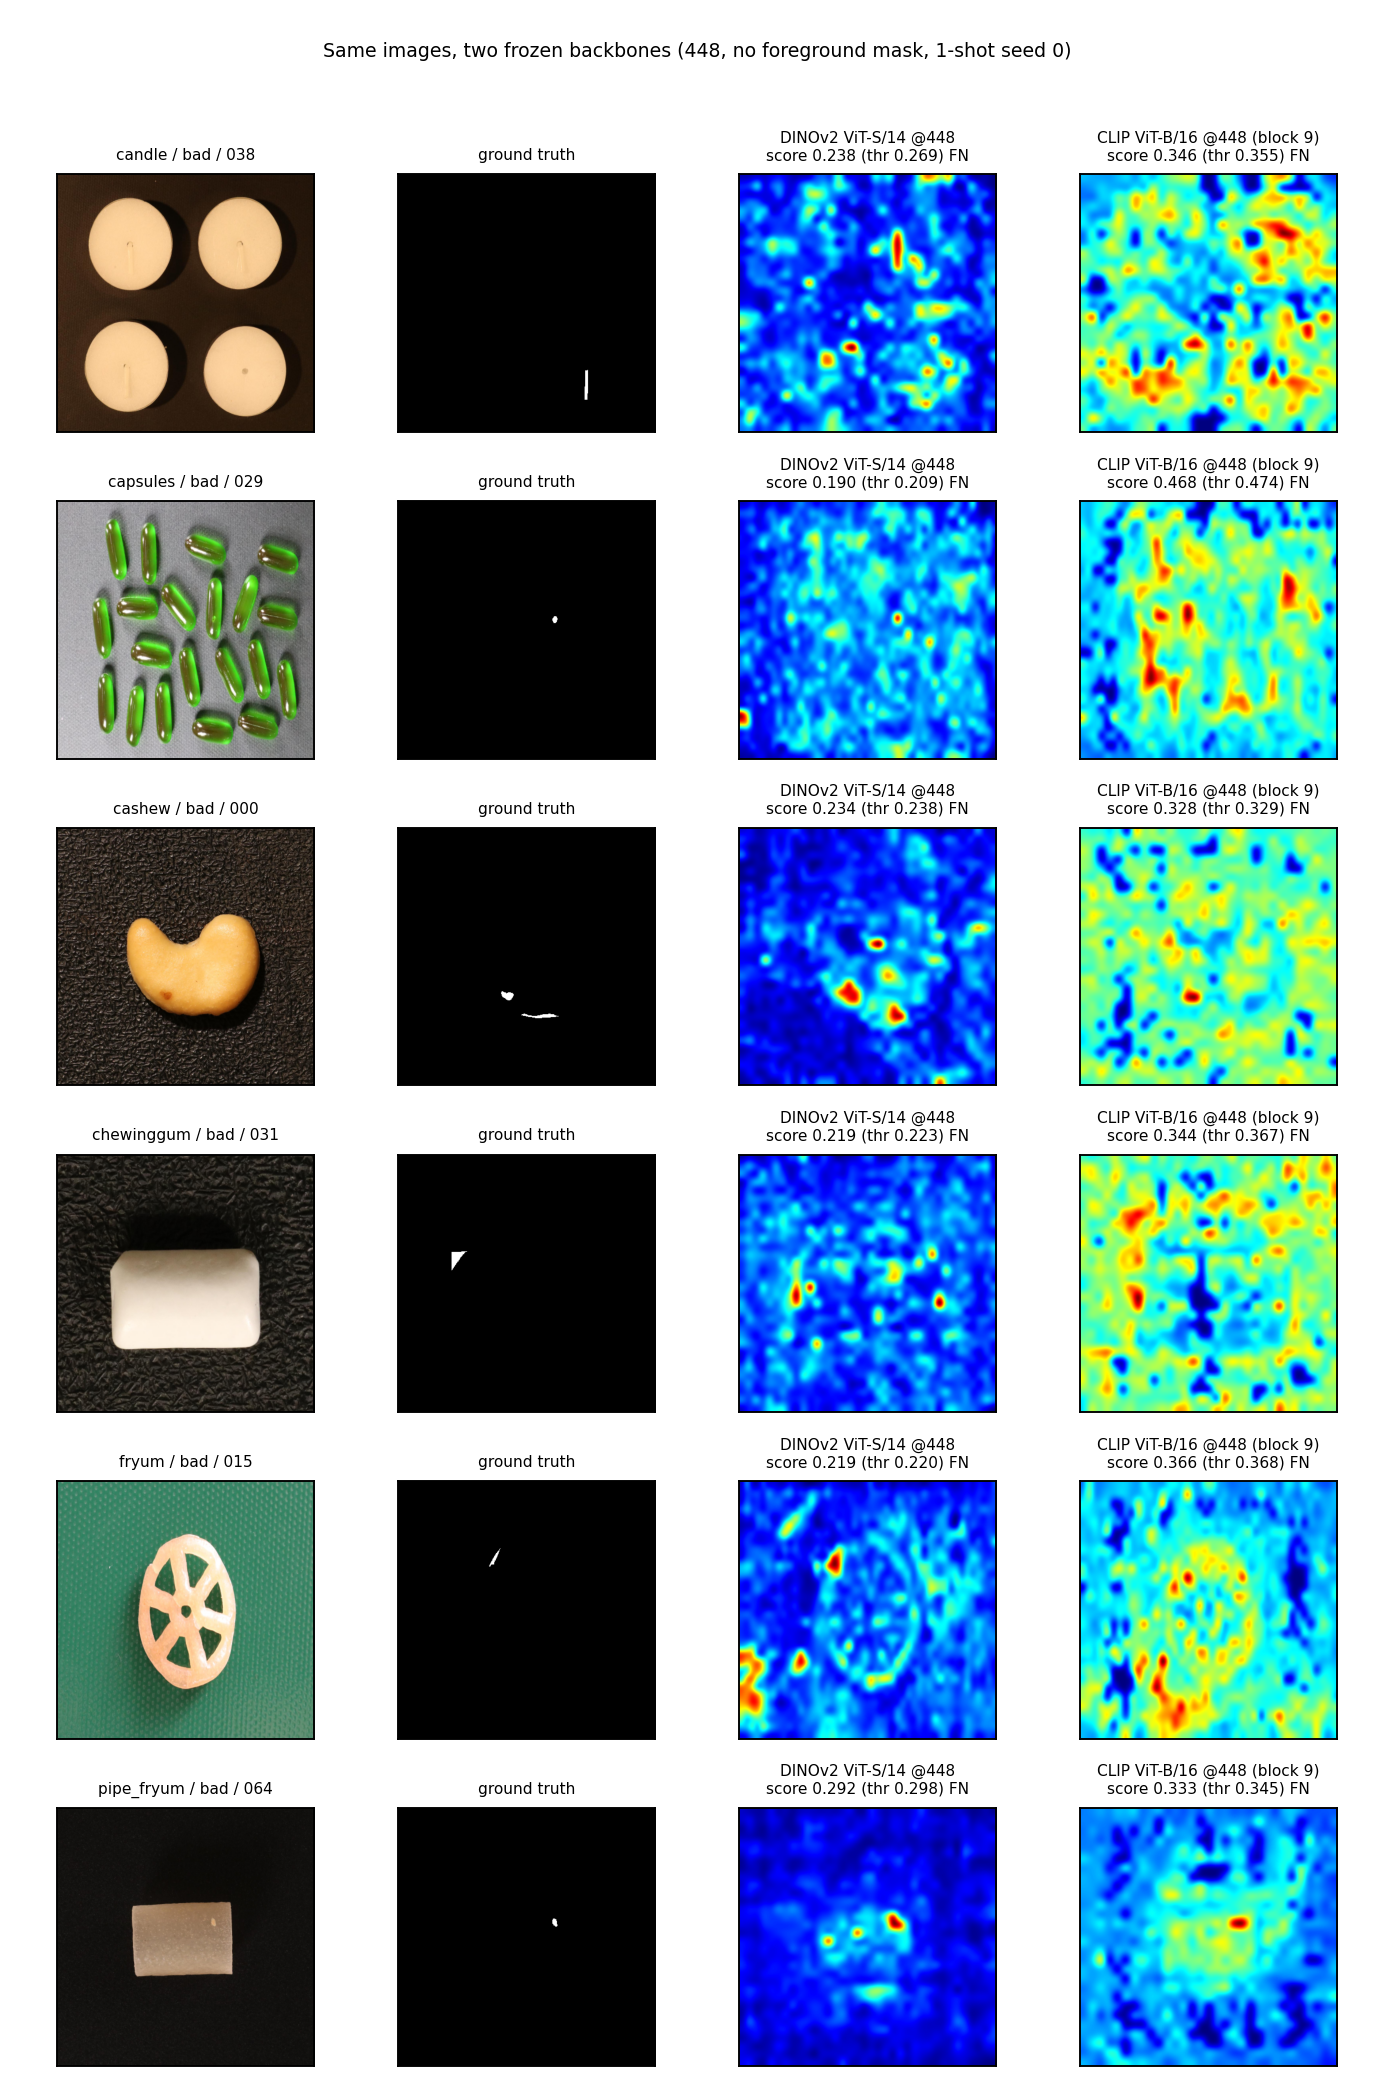
\includegraphics[width=0.94\columnwidth]{figures/heatmap_panel.png}
  \caption{Both-miss cases picked by a fixed rule before either map was inspected: ground
  truth (top), DINOv2 distance map (middle), CLIP block-9 map (bottom) for one image per
  category. DINOv2's field is flat with isolated hotspots; CLIP's is high-variance
  everywhere.}
  \label{fig:heatmaps}
\end{figure}

\subsection{Error taxonomy (1-shot, seed 0)}
\label{sec:exp-taxonomy}

Each test image receives a verdict from its own arm's calibration threshold; the two verdicts
are crossed image-by-image over all 960 test images
(Table~\ref{tab:taxonomy}).

\begin{table}[t]
\centering
\caption{Verdict crossing at each arm's own calibration threshold, 1-shot seed 0 (960 test
images). The fourth cell completes once the multimodal branch's per-image verdicts are in.}
\label{tab:taxonomy}
\footnotesize
\begin{tabular}{lrr}
\toprule
verdict cell & images & share \\
\midrule
both arms right & 607 & 63.2\% \\
only DINOv2 right & 193 & 20.1\% \\
only CLIP right & 58 & 6.0\% \\
both wrong & 102 & 10.6\% \\
\bottomrule
\end{tabular}
\end{table}

The arms agree on only 63.2\% of images. Defects missed by both: 90 of 600; normals flagged
by both: 12 of 360. CLIP is right on \textbf{58 images where DINOv2 is wrong} (35 of them on
candle and pipe\_fryum, the two categories where its deficit is smallest or reversed) -- a
concrete, countable complementarity that bounds any score-fusion gain from below and
motivates \S\ref{sec:exp-fusion}. \bsec{The fourth cell, ``only the VLM is right'', fills
from E2's per-image verdicts.}

\subsection{Score-level fusion of the visual pair -- machinery pilot}
\label{sec:exp-fusion}

\begin{table}[t]
\centering
\caption{Fusion machinery pilot (1-shot, seed 0; \emph{not} comparable with the three-seed
rows of Table~\ref{tab:image}). Fused $=\alpha z_{\mathrm{DINOv2}} + (1-\alpha)
z_{\mathrm{CLIP}}$ after per-category median/MAD standardisation on the 20 calibration
scores. $\alpha{=}1$/$\alpha{=}0$ reproduce the single branches exactly (max deviation 0.0).}
\label{tab:fusion}
\small
\begin{tabular}{lrrrrr}
\toprule
$\alpha$ (weight on DINOv2 $z$) & 0.00 & 0.25 & 0.50 & 0.75 & 1.00 \\
\midrule
image AUROC, macro (\%) & 85.97 & 91.61 & \best{93.75} & 94.05 & 93.11 \\
realised FPR at nominal 5\% & 14.2\% & 16.9\% & 17.5\% & 13.9\% & 9.4\% \\
\bottomrule
\end{tabular}
\end{table}

This subsection validates the fusion protocol before the multimodal branch lands; it must
not be read as a main result. With the pre-registered rule of \S\ref{sec:method-fusion}, the
fused scores on the 960 images of the 1-shot seed-0 cell give Table~\ref{tab:fusion} and
Fig.~\ref{fig:alpha}.

Two honest readings. \emph{Ranking}: at the pre-registered $\alpha = 0.5$ the fused score
beats the better single arm by $+0.64$ points (94.05 at $\alpha = 0.75$ is the sweep's
maximum and is reported as sensitivity only); the gain is bounded by the 58 ``only CLIP
right'' images and is consistent with the taxonomy. \emph{Reliability}: the realised
false-alarm rate at the nominal 5\% threshold is 9.4--17.5\% across $\alpha$, \emph{including
the single branches} -- 20 training-normal calibration images do not cover the variation of
the normal test images, so thresholds must be reported as achieved operating points, not
calibrated guarantees~\cite{guo2017calibration,geifman2017selective}.
\bsec{E3/E4 (DINOv2+Qwen, CLIP+Qwen) and E5 (cross-backbone fusion) upgrade this subsection
to a main result.}

\begin{figure}[t]
  \centering
  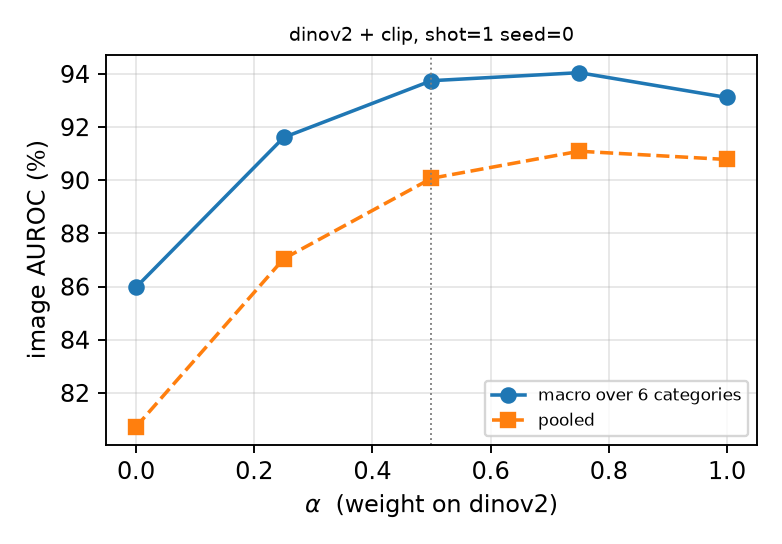
\includegraphics[width=0.94\columnwidth]{figures/fusion_visual_pair_1shot_seed0_alpha.png}
  \caption{Fusion sensitivity: image AUROC and realised false-alarm rate vs $\alpha$, visual
  pair, 1-shot seed 0. The pre-registered $\alpha=0.5$ is marked; the sweep maximum at
  $\alpha=0.75$ is reported as sensitivity only.}
  \label{fig:alpha}
\end{figure}

\subsection{Cost}
\label{sec:exp-cost}

Features are extracted exactly once per backbone and cached in float32; every (shot, seed)
cell afterwards is a $k$-NN pass, and the $\alpha$ sweep after that is offline and costs
milliseconds. Grid wall-clock on the shared RTX A6000 (with the $k$-NN search CPU-bound and
the GPU mostly idle): CLIP grid 265.6\,min, DINOv2 control ${\approx}4$\,h, stage-4 artefacts
(per-image dumps, heatmaps, taxonomy, tables, curves) ${\approx}27$\,min.

Per-image inference cost is measured separately at batch size 1
(Table~\ref{tab:cost}): end-to-end latency of one test image -- decode, resize/normalise,
upload, backbone forward, 1-NN over the reference bank, top-1\% pooling and the pixel-map
resize -- with feature extraction \emph{included} and the one-off reference-bank construction
amortised, plus peak CUDA memory on the same device.

\begin{table}[t]
\centering
\caption{Measured per-image inference cost (batch size 1, RTX A6000, faiss/BLAS threads
pinned to 1). Feature extraction included; reference-bank construction amortised; peak memory
from the CUDA allocator. \tbd{a}: paste from \texttt{scripts/bench\_inference.py};
\tbd{b}: measured by the multimodal branch's owner.}
\label{tab:cost}
\footnotesize
\setlength{\tabcolsep}{3.0pt}
\begin{tabular}{lrrr}
\toprule
Encoder & Lat.\ (ms) & Mem (MiB) & Par.\ (M) \\
\midrule
DINOv2 ViT-S/14 @448 & \tbd{a} & \tbd{a} & 22.1 \\
CLIP ViT-B/16 @448 L9 & \tbd{a} & \tbd{a} & 86.2 \\
Qwen-VL branch (E2) & \tbd{b} & \tbd{b} & \tbd{b} \\
\bottomrule
\end{tabular}
\end{table}

\subsection{Threats to validity}
\label{sec:exp-threats}

The controlled arms differ in patch size (14 vs 16\,px) and parameter count (22\,M vs 86\,M
vision parameters), so E1 measures \emph{this} CLIP encoder against \emph{this} DINOv2
encoder, not ``CLIP vs DINOv2'' in general; no patch-size-matched pair is publicly released.
CLIP runs at a resolution and normalisation different from its pretraining setup; the bicubic
position-table interpolation addresses this and is probe-verified but cannot be perfect. The
fusion pilot is one cell (1-shot, seed 0) of the two \emph{visual} arms; nothing in it may be
generalised until the per-(shot, seed) grid and the multimodal branch are in. Finally, all
six categories are object-centric product photographs; none of these conclusions should be
quoted for texture categories or scene-level anomalies, and MVTec AD~2's harder
scenarios~\cite{hecklerkram2026mvtec2} indicate the easier part of the problem space is what
we measure.
